%\documentclass[10pt]{article}
%
%\usepackage{tikz}
%\begin{document}
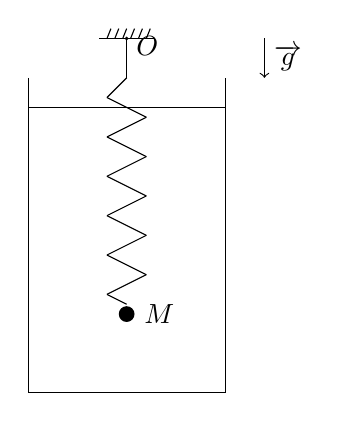
\begin{tikzpicture}[scale=.5]

\draw (0,8) -- (0,0) -- (5,0) -- (5,8);
\draw (0,7.25) -- (5,7.25);
\draw (1.8,9) -- (3.2,9);
\foreach \x in {0,.2,...,1}
{\draw (2+\x,9) -- (2.1+\x,9.25);}
\draw (2.5,9) -- (2.5,8);
\foreach \x in {1,2,...,5}
{\draw (2,8.5-\x) -- (3,8-\x);
\draw (3,8-\x) -- (2,7.5-\x);}
\draw (2,7.5) -- (2.5,8);
\draw (2,2.5) -- (2.5,2.25);
\fill (2.5,2) circle(.2) node at (2.7,2) [right]{$M$};
\draw[->] (6,9) -- (6,8) node[right,midway]{$\overrightarrow{g}$};
\fill (2.5,9) circle(.05) node at (2.5,8.8) [right]{$O$};


\end{tikzpicture}
%\end{document}
